\documentclass{beamer}
\usepackage{tikz}
\usepackage{euscript}
\usepackage{amsmath}
\usepackage{amssymb}
\usepackage{bm}
\usepackage{epsfig}
\usepackage{color} 
\usepackage{subfigure}
\usepackage{graphicx}
\usepackage[font=scriptsize,labelfont=scriptsize]{caption}
\usetikzlibrary{positioning,arrows,calc}
\newcommand{\tikzmark}[1]{\tikz[overlay,remember picture] \node (#1) {};}

\usefonttheme[onlymath]{serif}

\mode<presentation>
{
  \usetheme{Boadilla}
  \setbeamercovered{transparent}
}

\usepackage[english]{babel}
\usepackage[latin1]{inputenc}
\usepackage{times}
\usepackage[T1]{fontenc}

\newcommand{\norm}[2][]{\| #2 \|_{#1}}
\newcommand{\bftheta}{\mathbf{\theta}}
\newcommand{\bfv}{\mathbf{v}}
\newcommand{\bfx}{\mathbf{x}}

% Presentation Title
\title[Tree-Structured Wavelet CS]
{Tree-Structured Wavelet Compressive Sensing}

\subtitle{Based on a Paper by Lihan He and Lawrence Carin}

\author
{David A. Neal \and Josh Hunsaker}

\institute [USU]% (optional, but mostly needed)
{
  Advanced Digital Signal Processing  \\
  Electrical and Computer Engineering Dept. \\
  Utah State University \\[3em]
%

\includegraphics[width=1in]{idllogo3}
}


\date[] {}

\logo{
\includegraphics[height=1cm]{usu_logo_horizontal}\hspace{10cm}}


% Document Start
\begin{document}
\maketitle

%\begin{frame}
%  \frametitle{Topic Paper}
% This presentation presents theory and algorithms developed in
%  Exploiting Structure in Wavelet-Based Bayesian Compressive Sensing
%  by Lihan He and Lawrence Carin
%\end{frame}

\begin{frame}
  \frametitle{Overview}
  \begin{itemize}
    \setlength{\itemsep}{12pt}
  \item Compressive Sensing Background
  \item Wavelet Transforms
  \item Zero-Tree Structure
  \item Bayesian Inference
  \item Algorithm
  \item Results and Performance
   \end{itemize}
\end{frame}

\begin{frame}
  \frametitle{Compressive Sensing}
  \begin{itemize}
  \setlength{\itemsep}{15pt}
  \item Instead of sensing and then compressing, sense compressively
  \item Operates on the assumption of \emph{sparsity} in some basis
  \item Allows us to acquire significantly less data samples than the number of pixels in the image
   \end{itemize}
\end{frame}

\begin{frame}
  \frametitle{Compressive Sensing}
  \begin{equation*}
    \tikzmark{m1}\bfv = \underset{\tikzmark{m2}}{\Phi} \bftheta\tikzmark{m3}
    \begin{tikzpicture}[overlay, remember picture]
      \node[below of=m1,xshift=-3cm] (l1) {$\underset{N \times 1}{\text{\small Samples}}$};
      \draw[-,red] (l1) edge [->] (m1);
      \node[below of=m2,xshift=-0.5cm] (l2) {$\underset{N \times M}{\text{\small Sampling Matrix}}$};
      \draw[-,red] (l2) edge [->] (m2.north);
      \node[below of=m3,xshift=3cm] (l3) {$\underset{M \times 1}{\text{\small Wavelet Coefficients}}$};
      \draw[-,red] (l3) edge [->] (m3);
    \end{tikzpicture}
  \end{equation*}

  \vspace{1.5cm}
  \begin{itemize}
  \setlength{\itemsep}{15pt}
\item We are undersampled because $N \ll M$
  \item Reconstruction is possible via basis pursuit:
    \begin{equation*}
      \bftheta = \underset{\tilde{\bftheta}}{\arg \min} \,
      \norm[\ell_1]{\tilde{\bftheta}} \; s.t.\; \bfv =
      \Phi\tilde{\bftheta}
    \end{equation*}
  \end{itemize}
\end{frame}

\begin{frame}
  \frametitle{Wavelet Transforms}
  \begin{itemize}
    \setlength{\itemsep}{15pt}
    \item Wavelets provide a basis in which most natural images are sparse
    \item Wavelet transforms can be computed very quickly
    \item The wavelet basis matrix $\Psi$ computes a unitary transform:
  \end{itemize}
  \vspace{0.2cm}
  \begin{equation*}
    \tikzmark{m1}\bftheta = \underset{\tikzmark{m2}}{\Psi}^T \bfx\tikzmark{m3}
    \begin{tikzpicture}[overlay, remember picture]
      \node[below of=m1,xshift=-2.3cm] (l1) {$\underset{M \times 1}{\text{\small Wavelet Coefficients}}$};
      \draw[-,red] (l1) edge [->] (m1);
      \node[below of=m2] (l2) {$\underset{M \times M}{\text{\small Wavelet Basis}}$};
      \draw[-,red] (l2) edge [->] (m2.north);
      \node[below of=m3,xshift=2cm] (l3) {$\underset{M \times 1}{\text{\small Image Vector}}$};
      \draw[-,red] (l3) edge [->] (m3);
    \end{tikzpicture}
  \end{equation*}
\end{frame}

\begin{frame}
  \frametitle{Wavelet Transforms}

  \begin{figure}[]
    \centering
    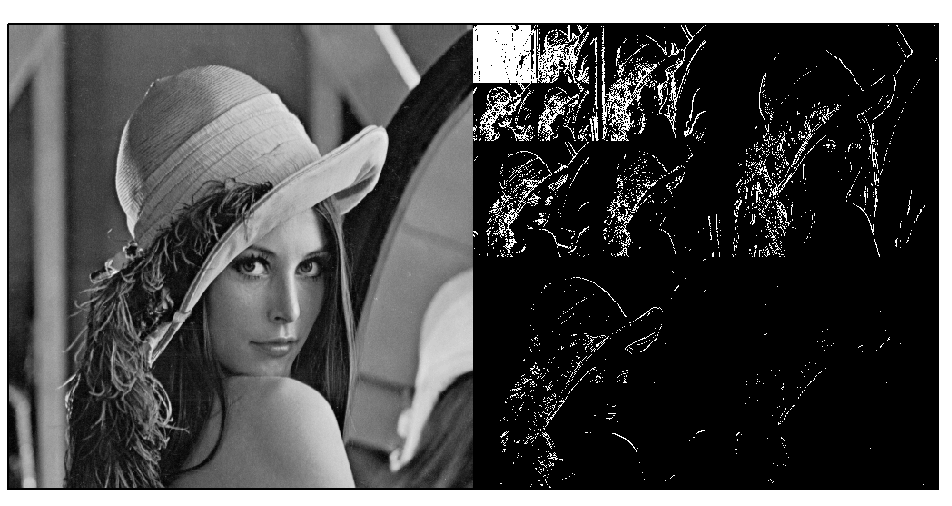
\includegraphics[width=12cm]{lenna_wavelet}
    \caption{A wavelet transform showing the significant components of $\bftheta$}
    \label{fig:lenna}
  \end{figure}
  
\end{frame}

\begin{frame}
  \frametitle{Zero-Tree Structure}
\begin{columns}
  \begin{column}{.5\linewidth}
    \begin{itemize}
      \setlength{\itemsep}{15pt}
    \item There is a parent-child relationship between scales
    \item The children of insignificant (small) coefficients are also small with high probability
    \item This structure can be exploited when trying to reconstruct $\bftheta$
      \end{itemize}    
    \end{column}
    \begin{column}{.5\linewidth}
      \begin{figure}[h!]
        \centering
        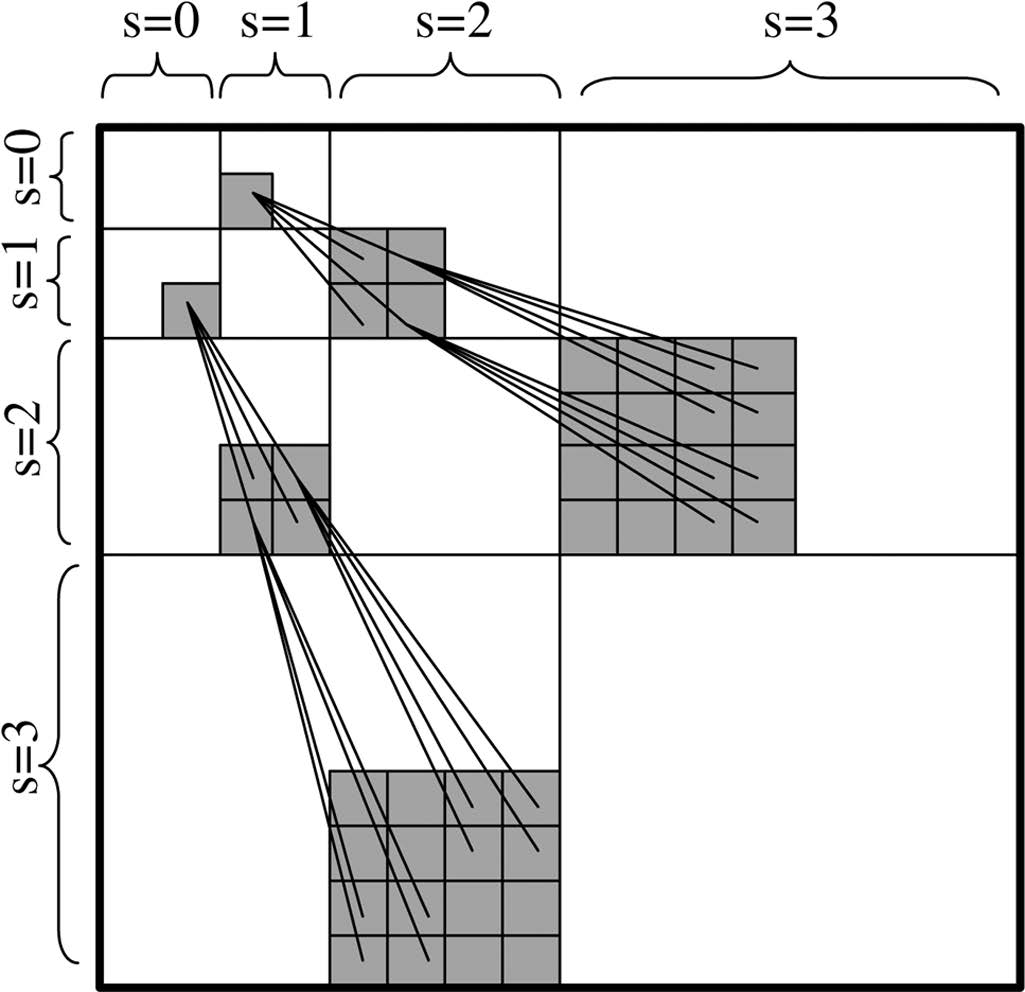
\includegraphics[width=5cm]{wavelet_tree}
        \caption{Wavelet decomposition showing the tree structure across scales}
        \label{fig:wavelet_tree}
      \end{figure}
    \end{column}
  \end{columns} 
\end{frame}

\begin{frame}
  \frametitle{Bayesian Inference}
  \begin{itemize}
  \item Another way to solve the problem is to utilize Bayes' rule and
    try Bayesian methods
  \item We want to find $\max p(\bftheta|v)$
  \item We do not know the distribution
    \begin{itemize}
      \item We can use Bayes' rule to find $p(\bftheta|v)
        \propto p(v|\bftheta)p(\bftheta)$
    \end{itemize}
  \item If we knew these distributions, we could try to directly
    solve
  \item Instead, we make some assumptions and use an iterative approach
  to solve for the maximizing value of $\bftheta$
  \end{itemize}
\end{frame}


\begin{frame}
  \frametitle{Bayesian Inference Assumptions}
  \begin{itemize}
  \item Assume that:
    \begin{itemize}
    \item $\theta_{s,i} \sim (1-\pi_{s,i})\delta_0 + \pi_{s,i} \mathcal{N}(0,\alpha_s^{-1})$
    \item $v|\bftheta, \alpha_n \sim
      \mathcal{N}(\Phi\bftheta,\alpha_n^{-1})$
    \end{itemize}
    \item with:
      \[   \pi_{s,i} = \left\{
      \begin{array}{ccc}
        \pi_r & if & s = 1  \\ 
        \pi_s^0 & if & 2 \leq s \leq L, \theta_{pa(s,i)} = 0  \\ 
        \pi_s^1 & if & 2 \leq s \leq L, \theta_{pa(s,i)} \neq 0 
      \end{array} \right. \]
      \[\begin{array}{cc}
      \alpha_ns \sim \Gamma(a_0,b_0) & \\
      \alpha_s \sim \Gamma(c_0,d_0) & s=1,\ldots,L \\
      \pi_r \sim \beta(e_0^r,f_0^r) & \\
      \pi_s^0 \sim \beta(e_0^{s0},f_0^{s0}) & s=2,\ldots,L \\
      \pi_s^1 \sim \beta(e_0^{s1},f_0^{s1}) & s=2,\ldots,L
      \end{array} \]
  \end{itemize}
\end{frame}

\begin{frame}
  \frametitle{Bayesian Inference Approach}
  \begin{itemize}
  \item Utilize conjugate priors to allow us to find the conditional
    posteriors analytically
  \item We can make use of Gibbs sampling to draw samples for each
    $\theta_{s,i}$, update the values for the mean, precision, and
    spike and slab parameter, and then draw new priors for the next iteration
  \item The prior updates exploit the zero tree structure to help
    choose parameters for the next iteration
  \item Due to ordering of $\theta_{s,i}$, we had to permute our
    coefficients when sampling so that the parent relationships
    matched up
   \end{itemize}
\end{frame}

%  EQUATIONS
\begin{frame}
  \frametitle{Bayesian Inference Model}
  \[       \begin{array}{ccc}
    p(\theta_{s,i}^{(j)}|-) & = &
    (1-\tilde{\pi}_{s,i}^{(j-1)})\delta_0+\tilde{\pi}_{s,i}^{(j-1)}\mathcal{N}(\tilde{\mu}_{s,i}^{(j-1)},1/\tilde{\alpha}_{s,i}^{(j-1)})
    \\
    & & \\
    \tilde{\alpha}_{s,i}^{(j)}) & = & \alpha_s^{(j-1)} + \alpha_n^{(j-1)}
    \mathbf{\phi}_m^T\mathbf{\phi}_m \\
    & & \\
    \tilde{\mu}_{s,i}^{(j)} & = &
    1/\tilde{\alpha}_{s,i}^{(j)}\alpha_n^{(j-1)}\mathbf{\phi}_m^T(\mathbf{v}-\sum_{k=1,k\neq
      m}^M\mathbf{\phi}_k\theta_k^{(j)}) \\
    & & \\
    \tilde{\pi}_{s,i}^{(j-1)} & = & 1, s = 0 \\
    & & \\
    \frac{\tilde{\pi}_{s,i}^{(j)}}{1-\tilde{\pi}_{s,i}^{(j)}} & =
    &
    \frac{\pi_{s,i}^{(j-1)}}{1-\pi_{s,i}^{(j-1)}}\frac{\mathcal{N}(0,1/\alpha_s^{(j-1)})}{\mathcal{N}(\tilde{\mu}_{s,i}^{(j)},1/\tilde{\alpha}_{s,i}^{(j)})},
    1 \leq s \leq L \\
  \end{array}
  \]
\end{frame}

\begin{frame}
  \frametitle{Bayesian Inference Model}
  \[       \begin{array}{ccc}
    p(\alpha_s^{(j)}|-) & = &  \Gamma(c_0+0.5\sum_{i=1}^{M_s}\mathbf{1}(\theta_{s,i}^{(j)}\neq
    0), d_0+0.5\sum_{i=1}^{M_s}\theta_{s,i}^{2,(j)})) \\
    & &  \\
    p(\pi_r^{(j)}|-) & = &
    \beta(e_0^r+\sum_{i=1}^{M_s}\mathbf{1}(\theta_{s,i}^{(j)}\neq
    0), f_0^r +\sum_{i=1}^{M_s}\mathbf{1}(\theta_{s,i}^{(j)}= 0)), s=1
    & & \\
    p(\pi_s^{0,(j)}|-) & = &
    \beta(e_s^{s0}+\sum_{i=1}^{M_s}\mathbf{1}(\theta_{s,i}^{(j)}\neq
    0,\theta_{pa(s,i)}^{(j)}= 0), \\
    & &  f_s^{s0} +\sum_{i=1}^{M_s}\mathbf{1}(\theta_{s,i}^{(j)}=
    0,\theta_{pa(s,i)}^{(j)}= 0)), 2 \leq s \leq L \\
    & & \\
    p(\pi_s^{(1,j)}|-) & = &
    \beta(e_s^{s1}+\sum_{i=1}^{M_s}\mathbf{1}(\theta_{s,i}^{(j)}\neq
    0,\theta_{pa(s,i)}^{1,(j)}\neq 0), \\
    & & f_s^{s1}+\sum_{i=1}^{M_s}\mathbf{1}(\theta_{s,i}^{(j)}=
    0,\theta_{pa(s,i)}^{(j)}\neq 0)), 2 \leq s \leq L \\
  \end{array}
  \]
\end{frame}

\begin{frame}
  \frametitle{Bayesian Inference Model}
  \begin{array}{ccc}
      p(\alpha_n^{(j)}|-) & = &
    \Gamma(a_0+N/2,b_0+\|(\mathbf{v}-\phi\mathbf{\theta}^{(j)})\|/2 
    & & \\
    \pi_{s,i}^{(j)} &= & \left\{ 
    \begin{array}{ccc}
      \pi_{sc} & if & s= 0 \\
      \pi_r^{(j)} & if & s = 1  \\ 
      \pi_s^{0,(j)} & if & 2 \leq s \leq L, \theta_{pa(s,i)} = 0  \\ 
      \pi_s^{1,(j)} & if & 2 \leq s \leq L, \theta_{pa(s,i)} \neq= 0 
    \end{array} \right. \\
  \end{array}
\end{frame}

\begin{frame}
  \frametitle{Bayesian Inference Model}
ADD MODEL GRAPH HERE
%  \begin{figure}
%    \centering
%    \includegraphics[width=.75\linewidth]{perfN2.eps}
%  \end{figure}
\end{frame}

\begin{frame}
  \frametitle{Algorithm}
  \begin{itemize}
  \item Initialize by picking random $\bftheta$ and using it to
    calculate and draw priors and other parameters
  \item Draw $\bftheta$
  \item Update mean, precision, and spike and slab parameter
  \item Draw new parameters for next iteration
  \item Repeat until convergence
  \end{itemize}
\end{frame}

\begin{frame}
  \frametitle{Results}
%   ADD PICTURE COMPARISON - ORIGINAL vs ours
% Do two of these?
\vspace{-1cm}
 \begin{figure}
    \centering
    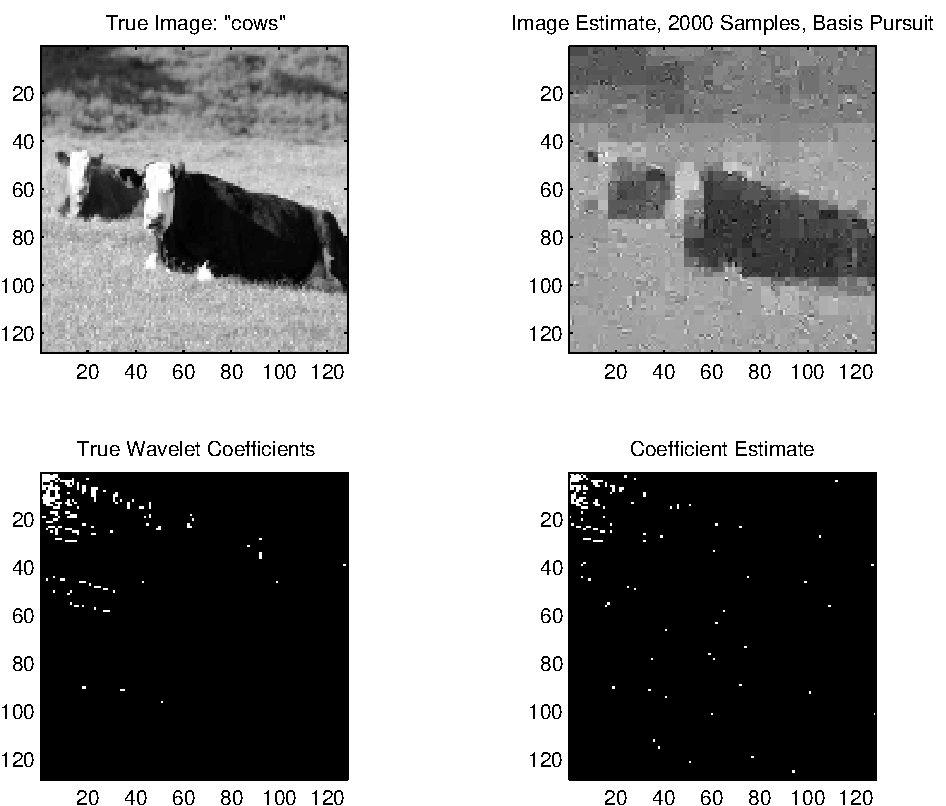
\includegraphics[width=.65\linewidth]{cows_m2000_cvx}
    \caption{Results of image reconstruction using basis pursuit from 2000 samples}
 \end{figure}
\end{frame}

\begin{frame}
  \frametitle{Performance Comparison}
 \begin{figure}
    \centering
    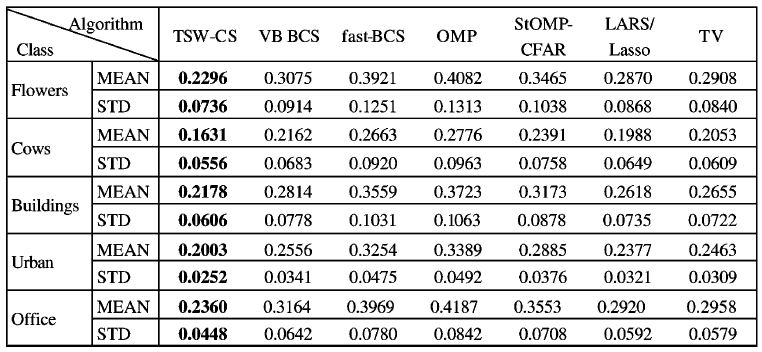
\includegraphics[width=.65\linewidth]{he_carin_results_m2000}
    \caption{Results from He and Carin paper}
 \end{figure}
\end{frame}

\begin{frame}
\frametitle{Conclusions}
\begin{itemize}
  \item Bayesian inference using Gibbs sampling is a viable
    alternative to convex optimization for compressive sensing
  \item Zero-tree structure can be exploited in the priors of the
    Bayesian approach
  \item The number of sensed samples can be reduced below that
    required for convex optimization
\end{itemize}
\end{frame}

%\begin{frame}
%\frametitle{Our Conclusions}
%\begin{itemize}
%  \item What did we learn?
%\end{itemize}
%\end{frame}

\end{document}
